\documentclass{beamer}
\usetheme{UASLP1}
\usepackage[utf8]{inputenc}
\usepackage[T1]{fontenc}
\usepackage{amsmath}
%% Use any fonts you like.
\usepackage{helvet}

\title{Grafos computacionales}
\subtitle{Redes Neuronales}
\author{Gamaliel Moreno Chávez}
\date{Enero-julio 2021}
\institute{\url{gamalielmch@uaz.edu.mx}}

\begin{document}
%%%%%%%%%%%%%%%%%%%%%%%%%%%%%%%%%%%%%%%%%%%%%%%%%%%%%%%%%%%
\begin{frame}[plain,t]
\titlepage
\end{frame}
%%%%%%%%%%%%%%%%%%%%%%%%%%%%%%%%%%%%%%%%%%%%%%%%%%%%%%%%%%%%%%%%%%
\begin{frame}{Contenido} 
   \tableofcontents
\end{frame}

%%%%%%%%%%%%%%%%%%55
\section{Grafos computacionales}
\begin{frame}
\frametitle{Grafos computacionales}
\begin{itemize}
\item Cálculo de $ J(\boldsymbol{\theta})$ y $\nabla_{\boldsymbol{\theta}}J(\boldsymbol{\theta})$ es complejo: Concatenación de productos matriz-vector, extensiones para el sesgo y funciones de activación no linenales constribuyen a complejidad.
\item En redes modernas, capas varían (función de activación, tipo, tamaño), lo que aumenta complejidad.
\item Redes clásicas: $ J(\boldsymbol{\theta})$ y $\nabla_{\boldsymbol{\theta}}J(\boldsymbol{\theta})$ calculados de previo y plasmados en código fijo para el caso concreto de $J$.
\item Marcos de trabajo (TensorFlow, Torch, ...) son flexibles: tipos de capas y funciones de activación se cambian fácilmente.
\item ¿cómo se pueden hacer los cálculos eficientemente?
\item¿cómo puedo agregar mis propios tipos de capas?
\end{itemize}
\end{frame}
%%%%%%%%%%%%%%%%%%%%%%%%%%%%%%%%%%%%%%%%%%%%%%%%%%%%%%%%%%%%%%%%%%
\begin{frame}
\frametitle{Grafos computacionales}
\begin{itemize}
\item Cálculo analítico y código correspondiente es complejo, tarda tiempo, y es poco reutilizable.  
\item Cálculo numérico del gradiente:
\begin{itemize}
\item es excesivamente caro
\item diferencias divididas requieren la evaluiación de $J$ 1 o 2 veces por cada parámetro escalar $ \boldsymbol{\theta}$
\item es muy fácil y rápido de implementar
\item se usa para verificar cálculo analítico
\end{itemize}

\item Alternativa: grafos computacionales: 

\begin{itemize}
\item Similar a la diferenciación automática
\item Aplican regla de la cadena para descomponer cálculo complejo en paso sencillos 
\item Compromiso entre los métodos numéricos y los métodos analíticos
\item Altamente flexibles
\end{itemize}

\end{itemize}
\end{frame}
%%%%%%%%%%%%%%%%%%%%%%%%%%%%%%%%%%%%%%%%%%%%%%%%%%%%%%%%%%%%%%%%%%
\section{Caso escalar}
\subsection{Propagación hacia adelante}
\begin{frame}
\frametitle{Grafos computacionales}
\begin{itemize}
\item idea:
\begin{enumerate}
\item Partir evaluación de una función en pasos elementales
\item Cada paso es un nodo del grafo
\item Relación entre pasos se expresa con aristas del grafo
\end{enumerate}
\item Explicaremos conceptos con ejemplo:
\begin{equation*}
f(x,\boldsymbol{\theta})=\frac{1}{1+e^{-\boldsymbol{\theta} x}}
\end{equation*}
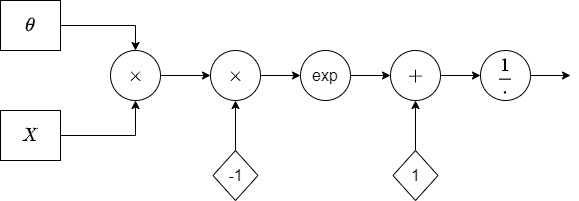
\includegraphics[scale=0.4]{im1}
\end{itemize}
\end{frame}
%%%%%%%%%%%%%%%%%%%%%%%%%%%%%%%%%%%%%%%%%%%%%%%%%%%%%%%%%%%%%%%%%%
\begin{frame}
\frametitle{Grafos computacionales}
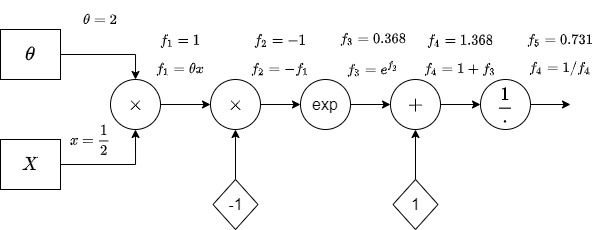
\includegraphics[scale=0.4]{im2}
\end{frame}
%%%%%%%%%%%%%%%%%%%%%%%%%%%%%%%%%%%%%%%%%%%%%%%%%%%%%%%%%%%%%%%%%%

\subsection{Propagación hacia atras}
\begin{frame}
\frametitle{Propagación hacia atrás}
\begin{itemize}
\item Buscamos ahora $dy/d\theta$ y $dy/dx$
 \item Esto se interpreta como el cambio en la salida debido a un cambio en la entrada
 \item La regla de la cadena subyace el cálculo nodo por nodo:
 \begin{equation*}
 \frac{\partial y}{\partial \theta}= \underbrace{\underbrace{\underbrace{\underbrace{\frac{\partial y}{\partial f_4}}_{b1} \cdot \frac{\partial f_4}{\partial f_3}}_{b2}\cdot \frac{\partial f_3}{\partial f_2}}_{b3} \cdot\frac{\partial f_2}{\partial f_1}}_{b4}\cdot \frac{\partial f_1}{\partial\theta}
 \end{equation*}
 \item Lo calculamos de atrás hacia adelante
\end{itemize}

\end{frame}
%%%%%%%%%%%%%%%%%%%%%%%%%%%%%%%%%%%%%%%%%%%%%%%%%%%%%%%%%%%%%%%%%%
\begin{frame}
\frametitle{Propagación hacia atrás}
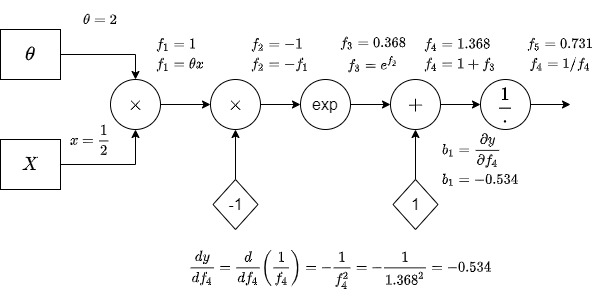
\includegraphics[scale=0.4]{im3}
\end{frame}
%%%%%%%%%%%%%%%%%%%%%%%%%%%%%%%%%%%%%%%%%%%%%%%%%%%%%%%%%%%%%%%%%%
\begin{frame}
\frametitle{Propagación hacia atrás}
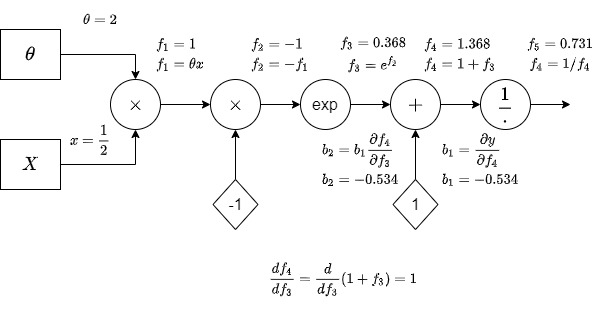
\includegraphics[scale=0.4]{im4}
\end{frame}
%%%%%%%%%%%%%%%%%%%%%%%%%%%%%%%%%%%%%%%%%%%%%%%%%%%%%%%%%%%%%%%%%%
\begin{frame}
\frametitle{Propagación hacia atrás}
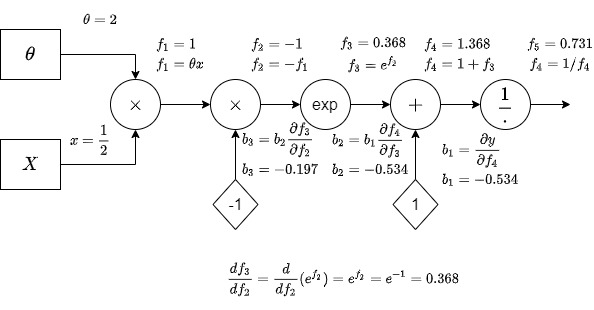
\includegraphics[scale=0.4]{im5}
\end{frame}
%%%%%%%%%%%%%%%%%%%%%%%%%%%%%%%%%%%%%%%%%%%%%%%%%%%%%%%%%%%%%%%%%%
\begin{frame}
\frametitle{Propagación hacia atrás}
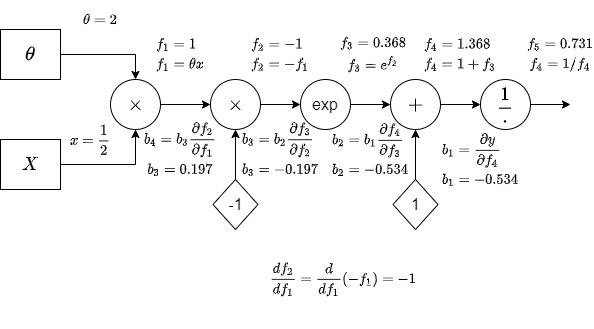
\includegraphics[scale=0.4]{im6}
\end{frame}
%%%%%%%%%%%%%%%%%%%%%%%%%%%%%%%%%%%%%%%%%%%%%%%%%%%%%%%%%%%%%%%%%%
\begin{frame}
\frametitle{Propagación hacia atrás}
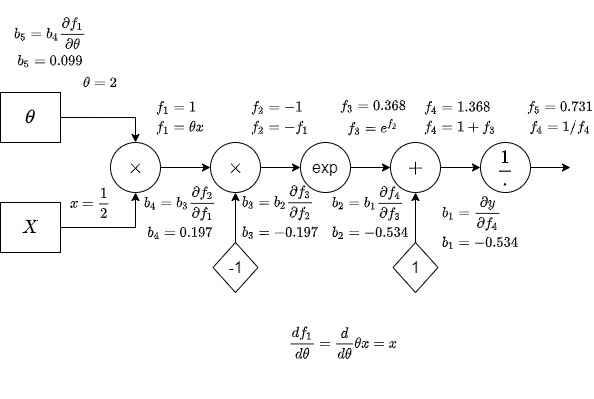
\includegraphics[scale=0.4]{im7}
\end{frame}
%%%%%%%%%%%%%%%%%%%%%%%%%%%%%%%%%%%%%%%%%%%%%%%%%%%%%%%%%%%%%%%%%%
\begin{frame}
\frametitle{Propagación hacia atrás}
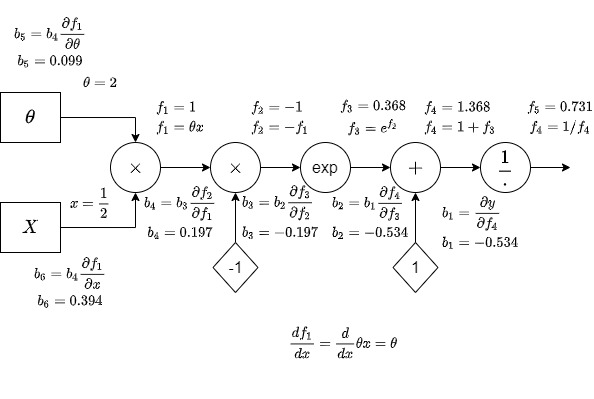
\includegraphics[scale=0.4]{im8}
\end{frame}
%%%%%%%%%%%%%%%%%%%%%%%%%%%%%%%%%%%%%%%%%%%%%%%%%%%%%%%%%%%%%%%%%%
\begin{frame}
\frametitle{Propagación hacia atrás}
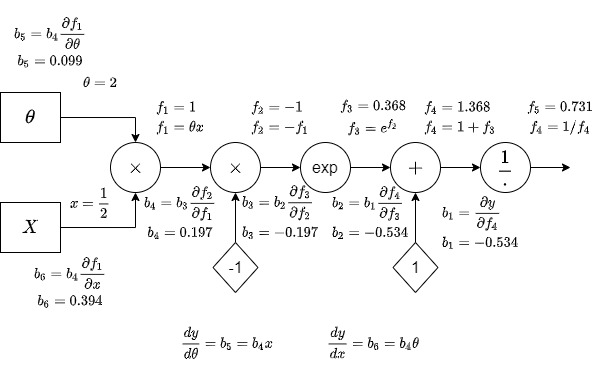
\includegraphics[scale=0.4]{im9}
\end{frame}
%%%%%%%%%%%%%%%%%%%%%%%%%%%%%%%%%%%%%%%%%%%%%%%%%%%%%%%%%%%%%%%%%%
\begin{frame}
\frametitle{Propagación hacia atrás}
\begin{itemize}
\item Obsérvese que claculamos $dy/d\theta$ y $dy/dx$
\item con eso, podemos adaptar las entradas en un proceso de descenso de gradiente:   
\begin{equation*}
\theta' \leftarrow \theta - \lambda \frac{\partial y}{\partial \theta} 
\end{equation*}
\begin{equation*}
x' \leftarrow x - \lambda \frac{\partial y}{\partial x} 
\end{equation*}
\item Estos cambios en $\theta$ y $x$ asegurarían que $y=f(x',\theta') \leq f(x\theta)$
\item La iteración de este proceso llevará hasta el mínimo (si $\lambda$ está bien elegido)
\end{itemize}
\end{frame}

%%%%%%%%%%%%%%%%%%%%%%%%%%%%%%%%%%%%%%%%%%%%%%%%%%%%%%%%%%%%%%%%%%

\subsection{Operación de un nodo}
\begin{frame}
\frametitle{Operación de un nodo}
\begin{itemize}
\item Comportamiento de nodos en escalares
\begin{itemize}
\item Múltiples entradas y una salida
\item Una entrada y múltiples salidas
\item Múltiples entradas y múltiples salidas 
\end{itemize}
\item Generalización a vectores y matrices
\end{itemize}
\end{frame}
%%%%%%%%%%%%%%%%%%%%%%%%%%%%%%%%%%%%%%%%%%%%%%%%%%%%%%%%%%%%%%%%%%
\begin{frame}
\frametitle{Operación de un nodo}
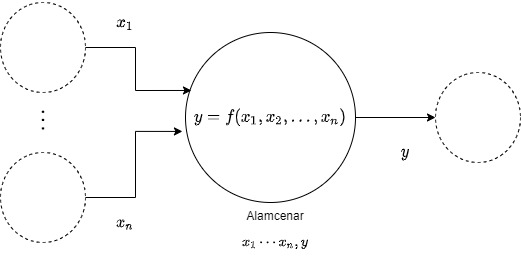
\includegraphics[scale=0.4]{im10}
\end{frame}
%%%%%%%%%%%%%%%%%%%%%%%%%%%%%%%%%%%%%%%%%%%%%%%%%%%%%%%%%%%%%%%%%%
\begin{frame}
\frametitle{Operación de un nodo}
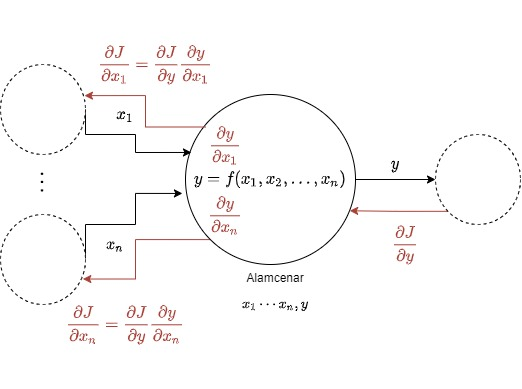
\includegraphics[scale=0.4]{im11}
\end{frame}
%%%%%%%%%%%%%%%%
%%%%%%%%%%%%%%%%%%%%%%%%%%%%%%%%%%%%%%%%%%%%%%%%%%%%%%%%%%%%%%%%%%
\begin{frame}
\frametitle{Operación de un nodo}
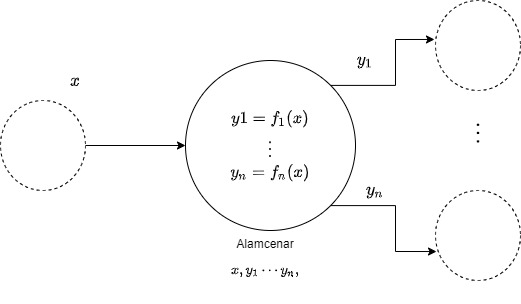
\includegraphics[scale=0.4]{im12}
\end{frame}
%%%%%%%%%%%%%%%%%%%%%%%%%%%%%%%%%%%%%%%%%%%%%%%%%%%%%%%%%%%%%%%%%%
\begin{frame}
\frametitle{Operación de un nodo}
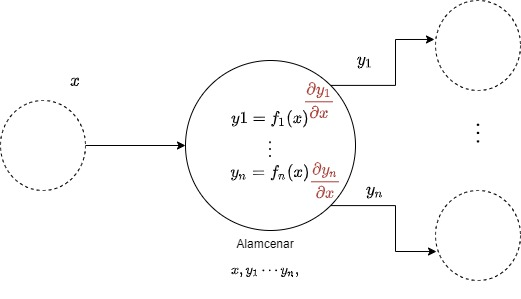
\includegraphics[scale=0.4]{im13}
\end{frame}
%%%%%%%%%%%%%%%%%%%%%%%%%%%%%%%%%%%%%%%%%%%%%%%%%%%%%%%%%%%%%%%%%%
\begin{frame}
\frametitle{Operación de un nodo}
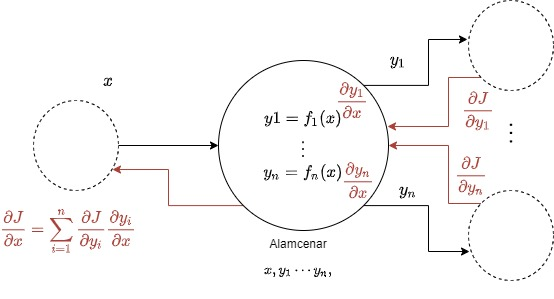
\includegraphics[scale=0.4]{im14}
\end{frame}
%%%%%%%%%%%%%%%%%%%%%%%%%%%%%%%%%%%%%%%%%%%%%%%%%%%%%%%%%%%%%%%%%%
\begin{frame}
\frametitle{Operación de un nodo}
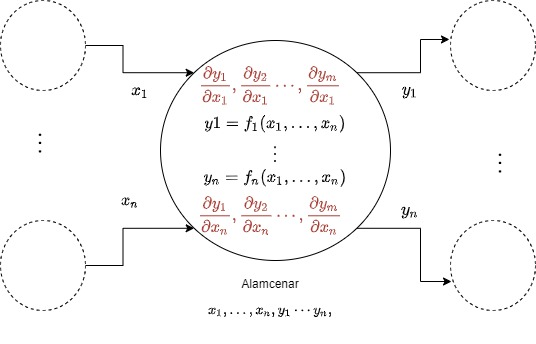
\includegraphics[scale=0.4]{im15}
\end{frame}
%%%%%%%%%%%%%%%%%%%%%%%%%%%%%%%%%%%%%%%%%%%%%%%%%%%%%%%%%%%%%%%%%%
\begin{frame}
\frametitle{Operación de un nodo}
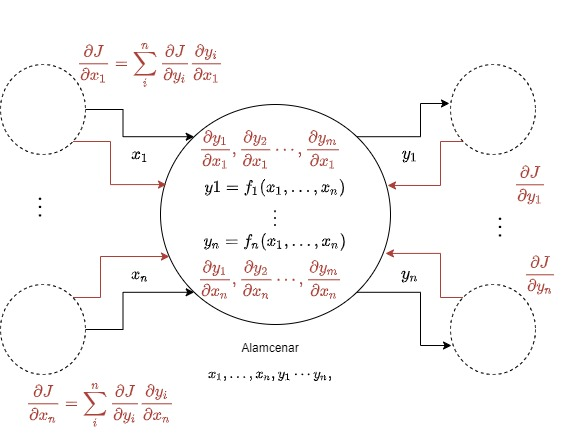
\includegraphics[scale=0.4]{im16}
\end{frame}
%%%%%%%%%%%%%%%%%%%%%%%%%%%%%%%%%%%%%%%%%%%%%%%%%%
\section{Caso vectorial}
\begin{frame}
\frametitle{Usando notación vectorial}
\begin{itemize}
\item El nodo anterior se simplifica usando notación vectorial  
\begin{align*} 
\boldsymbol{x} &= [x_1 \quad x_2 \cdots x_n]^T \\
\boldsymbol{y} &= [y_1 \quad y_2 \cdots y_m]^T = [f_1(\boldsymbol{x}) \quad f_2(\boldsymbol{x}) \cdots f_m(\boldsymbol{x})] \\
\end{align*}
\begin{equation*}
\nabla_{\boldsymbol{x}} J = \left[ \frac{\partial J}{\partial x_1}  \frac{\partial J}{\partial x_2} \cdots \frac{\partial J}{\partial x_n}   \right]^T  \quad \nabla_{\boldsymbol{y}} J= \left[ \frac{\partial J}{\partial y_1}  \frac{\partial J}{\partial y_2} \cdots \frac{\partial J}{\partial y_m}   \right]^T 
\end{equation*}
\begin{equation*}
\boldsymbol{D_xf}= 
\begin{bmatrix}
\nabla_{\boldsymbol{x}}^T f_1(\boldsymbol{x})\\
\nabla_{\boldsymbol{x}}^T f_2(\boldsymbol{x})\\
\vdots \\
\nabla_{\boldsymbol{x}}^T f_m(\boldsymbol{x})
\end{bmatrix}
= 
\begin{bmatrix}
\frac{\partial f_1}{\partial x_1} & \frac{\partial f_1}{\partial x_2} & \cdots & \frac{\partial f_1}{\partial x_n} \\
\frac{\partial f_2}{\partial x_1} & \frac{\partial f_2}{\partial x_2} & \cdots & \frac{\partial f_2}{\partial x_n}\\
\vdots &  \vdots & \ddots & \vdots \\
\frac{\partial f_m}{\partial x_1} & \frac{\partial f_m}{\partial x_2} & \cdot & \frac{\partial f_m}{\partial x_n}
\end{bmatrix}
\end{equation*}
\begin{equation*}
\nabla_{\boldsymbol{x}} J= \boldsymbol{D_x^T f} \nabla_{y} J
\end{equation*}
\end{itemize}
\end{frame}
%%%%%%%%%%%%%%%%%%%%%%%%%%%%%%%%%%%%%%%%%%%%%%%%%%%%%%%%%%%%%%%%%%
\begin{frame}
\frametitle{Operación de un nodo, vectorial}
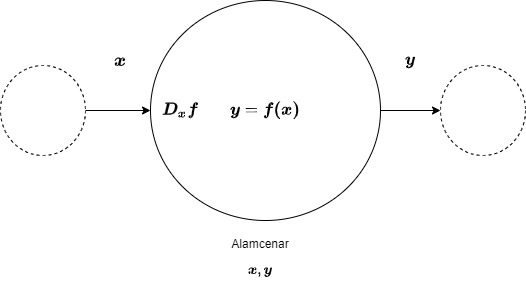
\includegraphics[scale=0.4]{im17}
\end{frame}
%%%%%%%%%%%%%%%%%%%%%%%%%%%%%%%%%%%%%%%%%%%%%%%%%%%%%%%%%%%%%%%%%%
\begin{frame}
\frametitle{Operación de un nodo, vectorial}
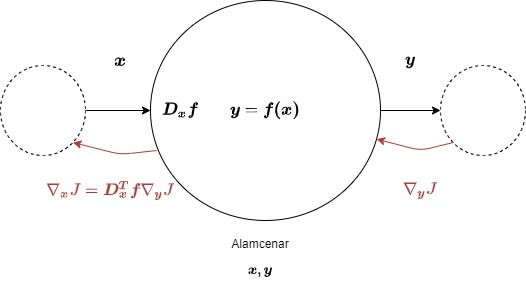
\includegraphics[scale=0.4]{im18}
\end{frame}
%%%%%%%%%%%%%%%%%%%%%%%%%%%%%%%%%%%%%%%%%%%%%%%%%%%%%%%%%%%%%%%%%%
\begin{frame}
\frametitle{Consideraciones prácticas}
\begin{itemize}
\item $\boldsymbol{D_x^T f}$ es el jacobiano de $\boldsymbol{f}$ respecto $\boldsymbol{x}$
\item La ecuación $\nabla_{\boldsymbol{x}} J= \boldsymbol{D_x^T f}\nabla_{\boldsymbol{y}} J$ integra todas las posibles influencias de cada salida y cada entrada, y aplica la regla de la cadena para ello.
\item con frecuencia sólo existen algunas dependencias y el Jacobiano  $\boldsymbol{D_x^T f}$ es disperso (tiene muchos ceros).
\begin{itemize}
\item Si $y_i$ solo depende de $x_i$ entonces el Jacobiano es diagonal.
\end{itemize}
\item En la práctica se calcula $\nabla_{\boldsymbol{x}} J$, que es lo que se retropropaga a los nodos precedentes.
\item Por eso el nombre: retro-propagación (backpropagation)
\end{itemize}

\end{frame}
%%%%%%%%%%%%%%%%%%%%%%%%%%%%%%%%%%%%%%%%%%%%%%%%%%%%%%%%%%%%%%%%%%
\begin{frame}
\frametitle{Generalización}
\begin{itemize}
\item Observe que $\boldsymbol{f(x)}$ puede ser cualquier función
\item $\boldsymbol{f(x)}$ agrupa varios cálculos en un nodo 
\item Granularidad según complejidad deseada para cada nodo
\item Resumiendo: cada nodo tiene tres tareas:
\begin{itemize}
\item propagar entrada a salida 
\item almacenar valores temporales para calcular gradientes
\item calcula gradiente de $J$ respecto a entradas del nodo, combinando información del gradiente $J$ respecto a las salidas y derivadas/gradientes de salidas respecto a entradas
\end{itemize}
\item Esto último es conceptual. En la práctica se resume el cálculo 
\item Si $\boldsymbol{x}$ o $\boldsymbol{y}$ fuese matrices, se analiza cada elemento de la matriz por separado, $\nabla_{\boldsymbol{x}} J$ o $\nabla_{\boldsymbol{y}} J$ serían matrices.
\end{itemize}

\end{frame}
%%%%%%%%%%%%%%%%%%%%%%%%%%%%%%%%%%%%%%%%%%%%%%%%%%%%%%%%%%%%%%%%%%
\begin{frame}
\frametitle{Ejemplo: Sigmoide}
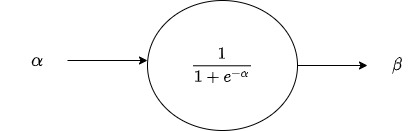
\includegraphics[scale=0.4]{im19}
\begin{itemize}
\item Entrada: $\alpha$
\item Salida: $\beta$
\item Cálculo en propagación hacia adelante: $\frac{1}{1+e^{-\alpha}}$
\item Cálculo en propagación hacia atrás: 
\begin{equation*}
\begin{split}
\frac{\partial \beta}{\partial \alpha} &=\frac{e^{-\alpha}}{(1+e-{\alpha})^2}= \frac{e^{-\alpha}}{(1+e-{\alpha})}+\frac{1}{(1+e-{\alpha})}\\
&=\frac{1+e^{-\alpha}-1}{(1+e-{\alpha})} \beta = \left( \frac{1+e^{-\alpha}}{1+e^{-\alpha}}- \frac{1}{1+e^{-\alpha}}\right)= (1-\beta ) \beta
\end{split}
\end{equation*}
\item Basta con almacenar $\beta$ para calcular $d\beta/d\alpha$
\end{itemize}
\end{frame}
%%%%%%%%%%%%%%%%%%%%%%%%%%%%%%%%%%%%%%%%%%%%%%%%%%%%%%%%%%%%%%%%%%
\begin{frame}
\frametitle{Ejemplo: Neurona totalmente conectada con sesgo}
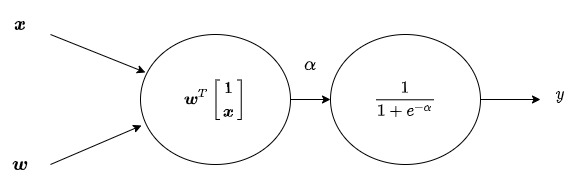
\includegraphics[scale=0.3]{im20}
\begin{itemize}
\item primer nodo extiende vector $\boldsymbol{x}$ con $1$ para poder aplicar el sesgo $w_0$ (primer componente de $\boldsymbol{w}$)
\begin{equation*}
\alpha = \begin{pmatrix}
w_0\\
+w_1 x_1\\
+w_2 x_2\\
\vdots \\
+w_n x_n
\end{pmatrix} \Rightarrow  \boldsymbol{D_{w}^T} \alpha = \nabla_{\boldsymbol{w}}\alpha = \begin{bmatrix} 1\\ \boldsymbol{x}\end{bmatrix} 
\end{equation*}
\begin{equation*}
  \boldsymbol{D_{x}^T} \alpha = \nabla_{\boldsymbol{x}}\alpha=\boldsymbol{w}= \begin{pmatrix}
w_1 \\ w_2 \\ \vdots \\ w_n  \end{pmatrix}
\end{equation*}

\end{itemize}

\end{frame}
%%%%%%%%%%%%%%%%%%%%%%%%%%%%%%%%%%%%%%%%%%%%%%%%%%%%%%%%%%%%%%%%%%
\begin{frame}
\frametitle{Ejemplo: Neurona totalmente conectada con sesgo}
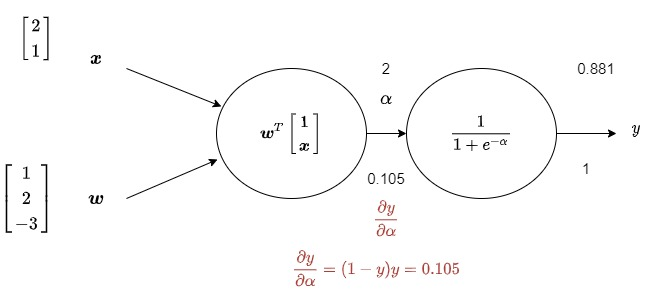
\includegraphics[scale=0.4]{im21}
\end{frame}
%%%%%%%%%%%%%%%%%%%%%%%%%%%%%%%%%%%%%%%%%%%%%%%%%%%%%%%%%%%%%%%%%%
\begin{frame}
\frametitle{Ejemplo: Neurona totalmente conectada con sesgo}
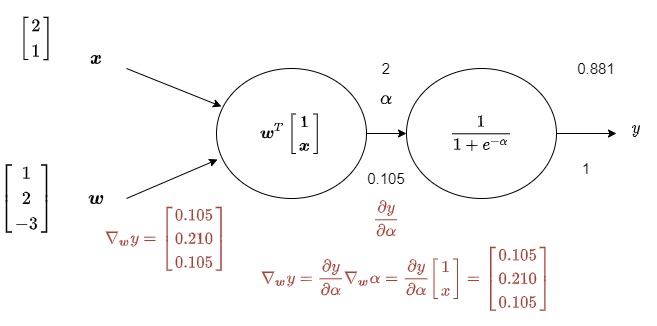
\includegraphics[scale=0.4]{im22}
\end{frame}
%%%%%%%%%%%%%%%%%%%%%%%%%%%%%%%%%%%%%%%%%%%%%%%%%%%%%%%%%%%%%%%%%%
\begin{frame}
\frametitle{Ejemplo: Neurona totalmente conectada con sesgo}
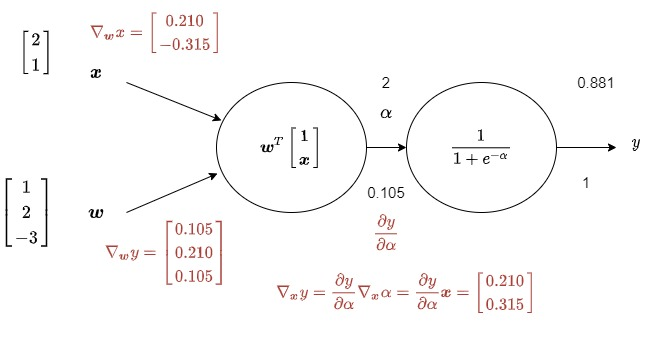
\includegraphics[scale=0.4]{im23}
\end{frame}
%%%%%%%%%%%%%%%%%%%%%%%%%%%%%%%%%%%%%%%%%%%%%%%%%%%%%%%%%%%%%%%%%%
\begin{frame}
\frametitle{Compuertas}
\begin{itemize}
\item Los nodos de un grafo computacional se comportan como compuertas
\item A continuación se analizarán algunos casos comunes
\end{itemize}
\end{frame}
%%%%%%%%%%%%%%%%%%%%%%%%%%%%%%%%%%%%%%%%%%%%%%%%%%%%%%%%%%%%%%%%%%
\begin{frame}
\frametitle{Compuertas}
\begin{itemize}
\item Los nodos de un grafo computacional se comportan como compuertas
\item A continuación se analizarán algunos casos comunes
\end{itemize}
\end{frame}
%%%%%%%%%%%%%%%%%%%%%%%%%%%%%%%%%%%%%%%%%%%%%%%%%%%%%%%%%%%%%%%%%%
\begin{frame}
\frametitle{Suma}

\begin{itemize}
\item La suma distribuye el gradiente a todas las entradas
\end{itemize}
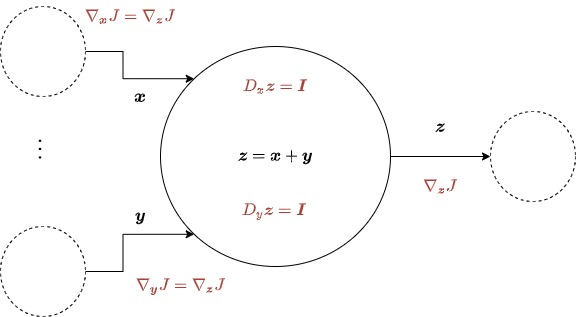
\includegraphics[scale=0.35]{im24}
\end{frame}
%%%%%%%%%%%%%%%%%%%%%%%%%%%%%%%%%%%%%%%%%%%%%%%%%%%%%%%%%%%%%%%%%%
\begin{frame}
\frametitle{Máximo}

\begin{itemize}
\item El nodo $z=max(x,y)$ produce el máximo de variables de entrada
\item la pregunta es ¿qué hace la derivada?
\item la interpretación es la siguiente
\begin{itemize}
\item si $x>y$, entonces $z=x$ y por tanto $\frac{\partial z}{\partial x}=1$ y $\frac{\partial z}{\partial y}=0$
\item si $x<y$, entonces $z=y$ y por tanto $\frac{\partial z}{\partial x}=0$ y $\frac{\partial z}{\partial y}=1$
\end{itemize}
\item La compuerta $max$ enruta entonces el gradiente por aquella entrada con el máximo valor
\item Esto se generaliza fácilmente a vectores componente por componente.
\end{itemize}
\end{frame}
%%%%%%%%%%%%%%%%%%%%%%%%%%%%%%%%%%%%%%%%%%%%%%%%%%%%%%%%%%%%%%%%%%
\begin{frame}
\frametitle{Máximo}
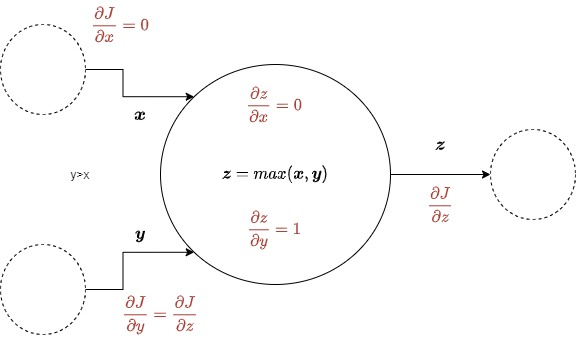
\includegraphics[scale=0.35]{im25}
\end{frame}
%%%%%%%%%%%%%%%%%%%%%%%%%%%%%%%%%%%%%%%%%%%%%%%%%%%%%%%%%%%%%%%%%%
\begin{frame}
\frametitle{Conmutadores}
\begin{itemize}
\item Los distintos tipos de producto intercambian de algún modo u otro las entradas en la propagación hacia atrás. 
\item Solo en algunos casos es posible calcular el jacobiano
\item A continuación analizaremos cuatro casos:
\begin{itemize}
\item Producto de dos escalares $z=xy$
\item Producto interno de dos vectores $z= \boldsymbol{x}^T\boldsymbol{y}$
\item Producto externo de dos vectores $\boldsymbol{Z}= \boldsymbol{x}\boldsymbol{y}^T$
\item Producto de dos matrices $\boldsymbol{Z}= \boldsymbol{X}\boldsymbol{Y}$
\end{itemize}
\end{itemize}
\end{frame}
%%%%%%%%%%%%%%%%%%%%%%%%%%%%%%%%%%%%%%%%%%%%%%%%%%%%%%%%%%%%%%%%%%
\begin{frame}
\frametitle{Producto escalar}
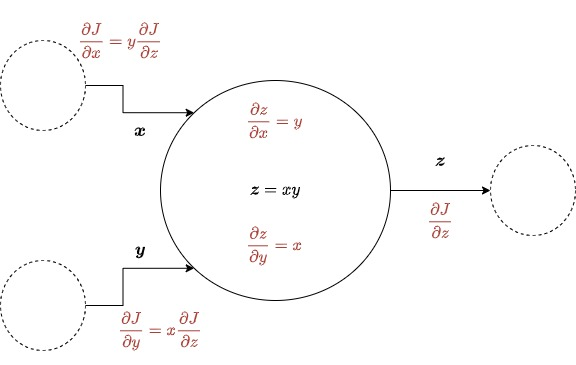
\includegraphics[scale=0.35]{im26}
\end{frame}
%%%%%%%%%%%%%%%%%%%%%%%%%%%%%%%%%%%%%%%%%%%%%%%%%%%%%%%%%%%%%%%%%%
\begin{frame}
\frametitle{Producto interno de dos vectores}
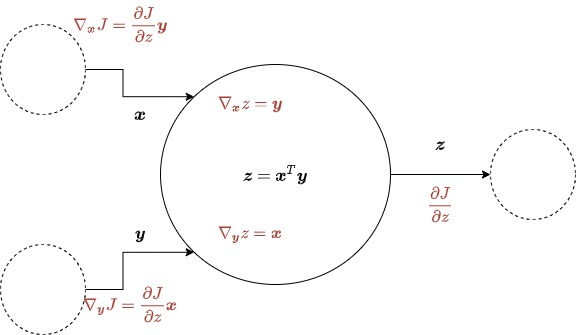
\includegraphics[scale=0.35]{im27}
\end{frame}
%%%%%%%%%%%%%%%%%%%%%%%%%%%%%%%%%%%%%%%%%%%%%%%%%%%%%%%%%%%%%%%%%%
\begin{frame}
\frametitle{Producto interno de dos vectores}
\begin{itemize}
\item El producto externo produce una matriz a la salida
\item Supongamos $\boldsymbol{x}\in \mathbb{R}^{n}$ e $\boldsymbol{y} \in \mathbb{R}^{m}$
\begin{equation*}
\boldsymbol{Z}= \begin{bmatrix}
z_{11} & z_{12} & \cdots & z_{1m}\\
z_{21} & z_{22} & \cdots & z_{2m}\\
\vdots & \vdots & \ddots & \vdots \\
z_{n1} & z_{n2} & \cdots & z_{nm}
\end{bmatrix} =\boldsymbol{xy}^T= \begin{bmatrix}
x_1y_1 & x_1y_2 & \cdots & x_1y_m\\
x_2y_1 & x_2y_2 & \cdots & x_2y_m\\
\vdots & \vdots & \ddots & \vdots \\
x_ny_1 & x_ny_2 & \cdots & x_ny_m
\end{bmatrix}
\end{equation*}
\item siguendo el principio de múltiples salidas (elementos de $\boldsymbol{Z}$)
\begin{equation*}
\frac{\partial J}{\partial x_k}=\sum_i\sum_j \frac{\partial J}{\partial z_{ij}}\frac{\partial z_{ij}}{\partial x_k}= \sum_i\sum_j \frac{\partial J}{\partial z_{ij}} \frac{\partial {(x_iy_j)}}{\partial x_k}
\end{equation*}
donde solo los términos con $i=k$ sobreviven 
\begin{equation*}
\frac{\partial J}{\partial x_k}=\sum_j\frac{\partial J}{\partial z_{kj}}y_j \Rightarrow \nabla_{\boldsymbol{x}}J=\nabla_{\boldsymbol{z}} J \boldsymbol{y}
\end{equation*}
\end{itemize}
\end{frame}
%%%%%%%%%%%%%%%%%%%%%%%%%%%%%%%%%%%%%%%%%%%%%%%%
\ThankYouFrame
%%%%%%%%%%%%%%%%%%%%%%%%%%%%%%%%%%%%%%%%%%%%%%%%%%%%%%%%%%%%%%%%%%

\end{document}
